\documentclass[12pt]{article}
\usepackage[margin=1in]{geometry}
\usepackage{graphicx}
\usepackage{setspace}
\usepackage{caption}

% Support compilation from the repository root or from memo/.
% Missing generated results are an error, never a reason to use old literal values.
\IfFileExists{memo/ED_memo.tex}{%
    \newcommand{\ResultsFile}{memo/results.tex}%
    \graphicspath{{figure/}}%
}{%
    \newcommand{\ResultsFile}{results.tex}%
    \graphicspath{{../figure/}}%
}
\InputIfFileExists{\ResultsFile}{}{% 
    \PackageError{ED-memo}{Generated results.tex is missing}%
    {Run python script/plot.py from the repository root, then compile again.}%
}

\begin{document}

\noindent
\textbf{DATE:} \today \\
\textbf{SUBJECT:} Analysis of 2-Year Public Enrollment Trends and Federal Grant Allocation \\
\normalsize

\subsection*{Executive Summary}
\begin{itemize}
    \item Enrollment: First-time, full-time undergraduate enrollment at public two-year colleges changed by \EnrollmentChangePct{}\% between \StudyStartYear{} and \StudyEndYear{} in the retained panel.
    \item Grant allocation: The observed and simulated cross-state 90/10 ratios are \CurrentAidRatio{} and \SimulatedAidRatio{}, respectively. The simulated budget change in the retained sample is \$\BudgetChangeMillions{} million.
\end{itemize}

\subsection*{Data \& Methodology}
The complete-case balanced panel contains \PanelInstitutions{} undergraduate institutions and \PanelRows{} institution-year observations from unrevised IPEDS files. Institutions without all required eligible observations are excluded, so results describe only the retained sample.

\subsection*{2-Year Public College Enrollment Trends}
Total first-time, full-time enrollment across public two-year colleges was \EnrollmentStart{} in \StudyStartYear{} and \EnrollmentEnd{} in \StudyEndYear{}, a change of \EnrollmentChangePct{}\% (Figure~\ref{fig:enrollment}).

\subsection*{Current Federal Grant Distribution (\AidAcademicYear)}
Average federal grant aid per student was \$\NYAid{} in New York and \$\VTAid{} in Vermont (Figure~\ref{fig:ny-vt}). Across the \PanelStates{} included states, the unweighted mean of state rates was \$\CurrentAidMean{}, the sample standard deviation was \$\CurrentAidSD{}, and the 90/10 ratio was \CurrentAidRatio{} (Figure~\ref{fig:state-aid}). Each state rate is total grants divided by total enrollment within that state.

\subsection*{Simulated Policy Impact}
Under the specified institution-level formula, the observed and simulated standard deviations of state aid rates are \$\CurrentAidSD{} and \$\SimulatedAidSD{}, respectively. The corresponding highest-minus-lowest ranges are \$\CurrentAidRange{} and \$\SimulatedAidRange{}, and the 90/10 ratios are \CurrentAidRatio{} and \SimulatedAidRatio{} (Figures~\ref{fig:simulated-aid} and~\ref{fig:policy-spread}). Simulated minus observed spending is \$\BudgetChangeDollars{} in the retained sample.

\subsection*{Conclusion}
The simulated budget difference is \$\BudgetChangeMillions{} million; positive values indicate additional spending and negative values indicate lower spending. Figure~\ref{fig:winners-losers} shows states with increases and decreases in simulated grant totals. These calculations describe allocation and dispersion, not causal effects or a welfare assessment.

\clearpage
\section*{Appendix: Figures}

\begin{figure}[htbp]
    \centering
    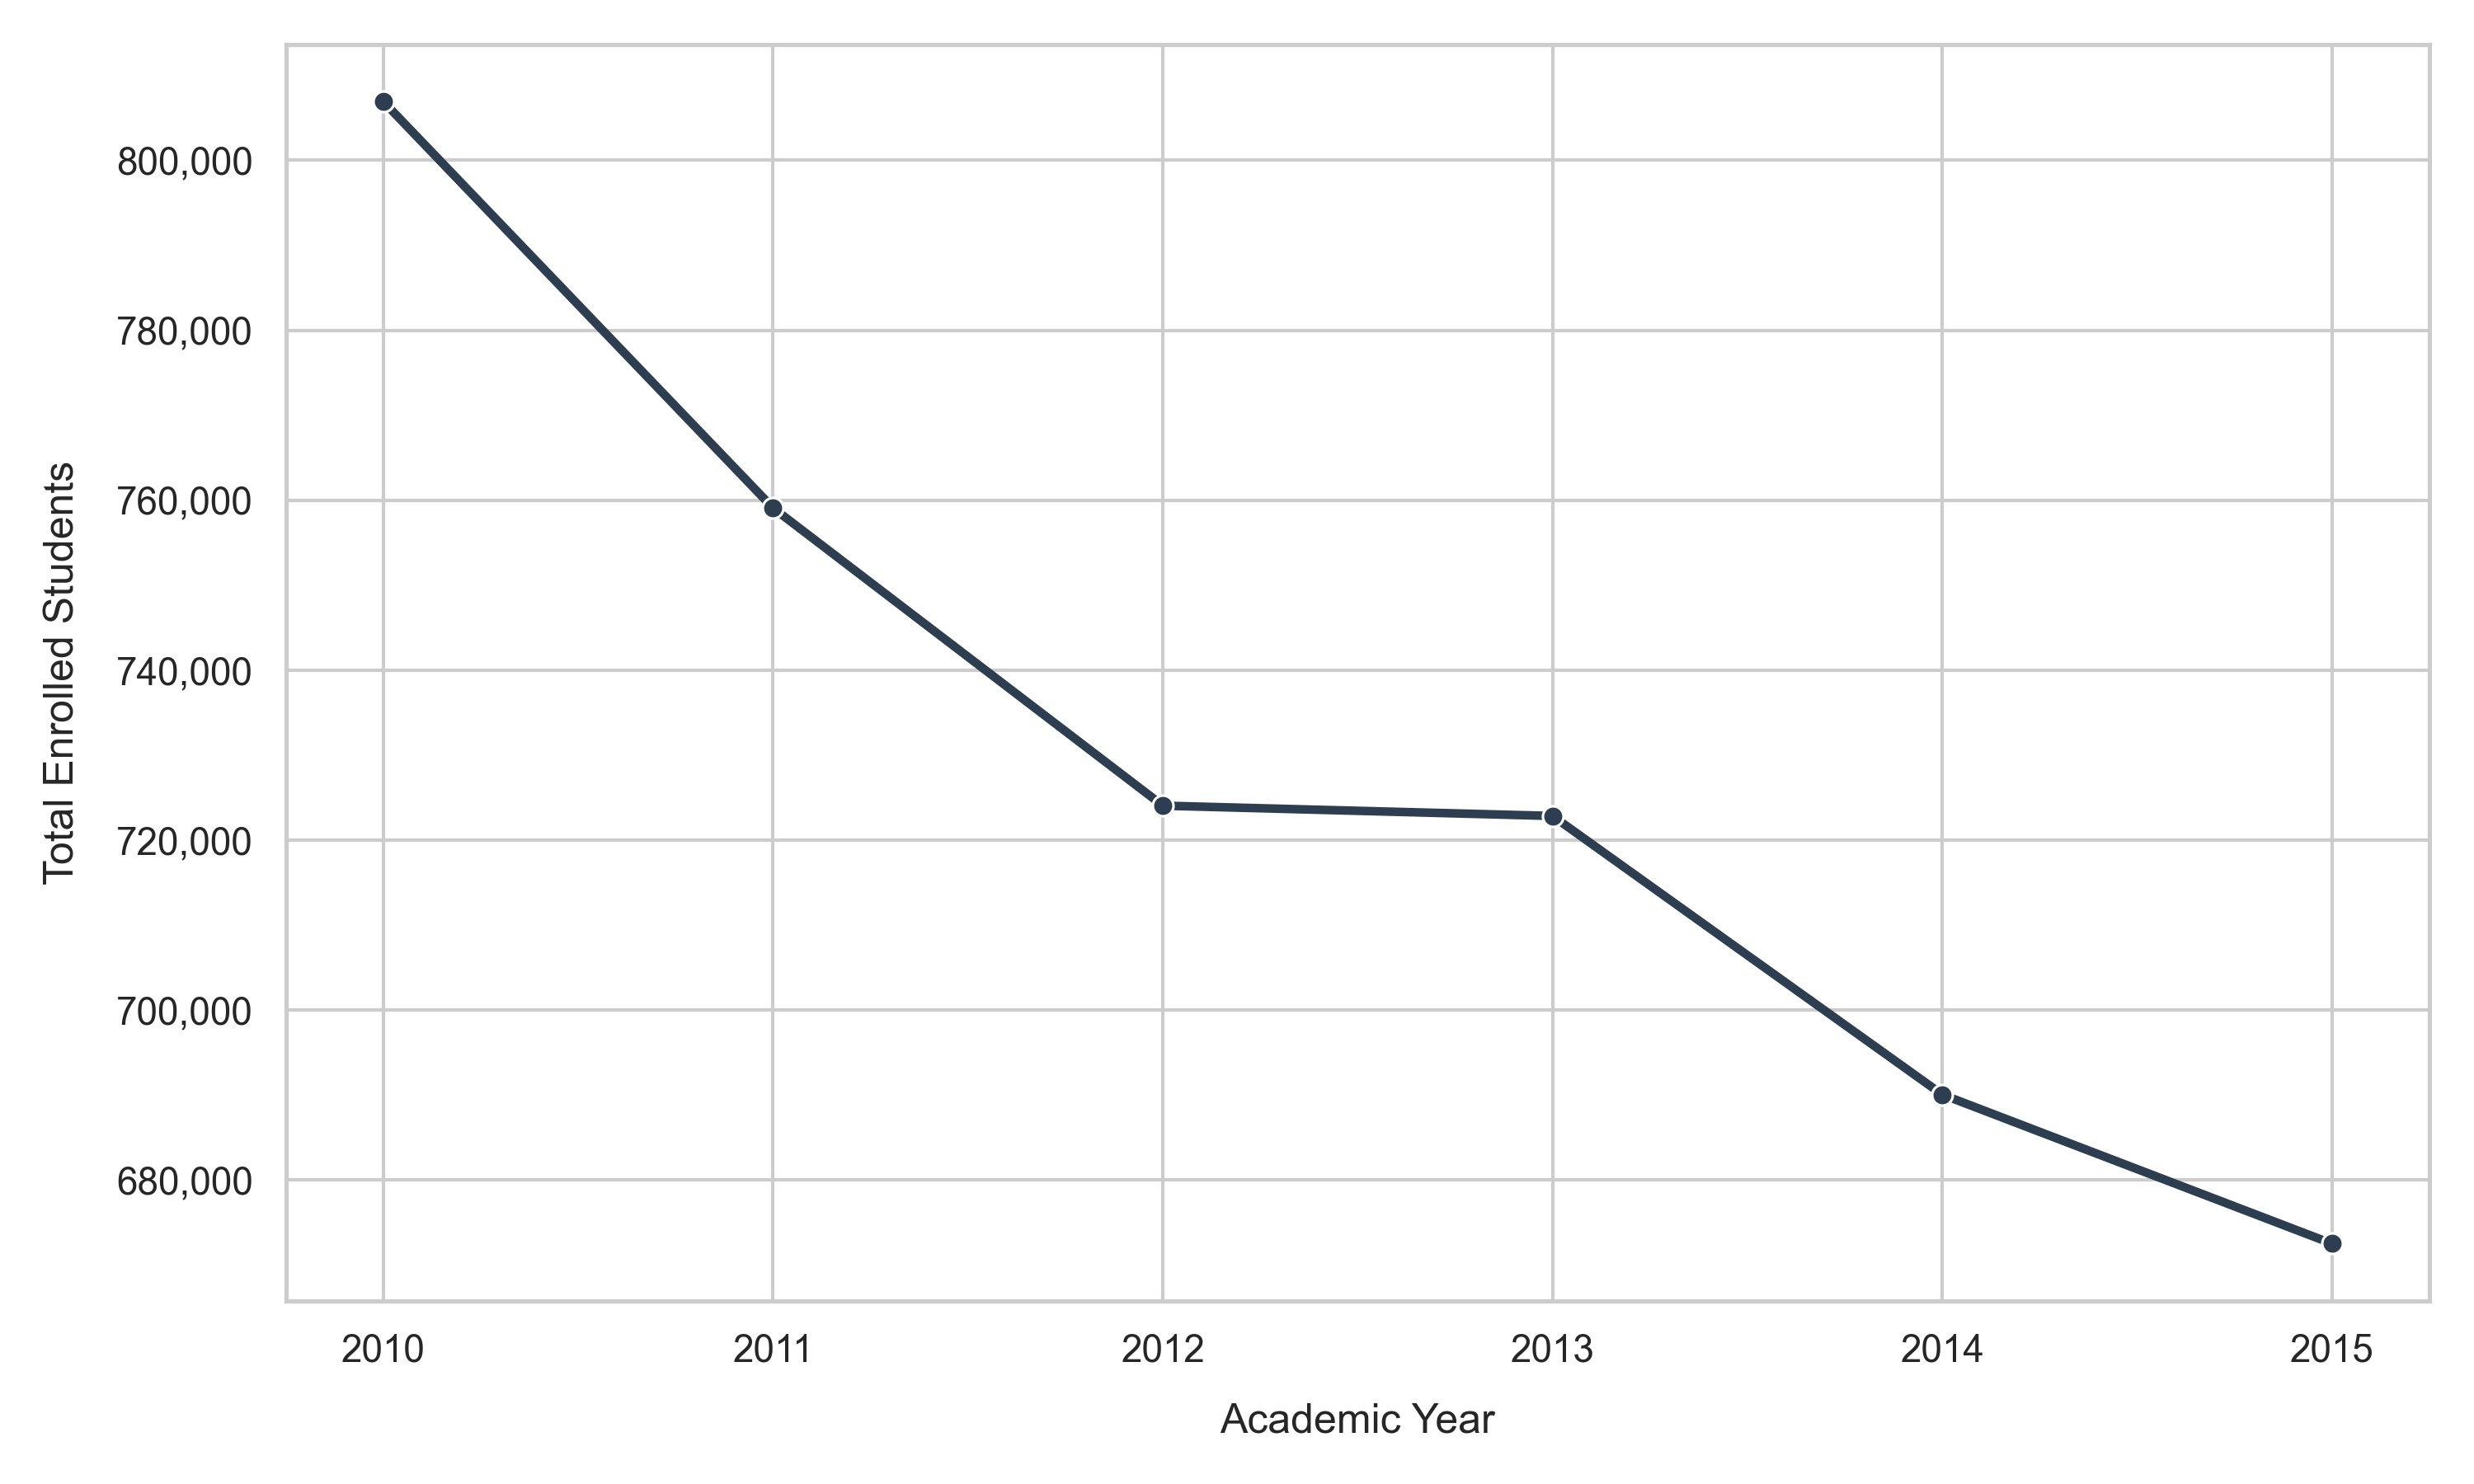
\includegraphics[width=\linewidth]{figure1_2yr_enrollment.png}
    \caption{Total First-Time, Full-Time Undergraduate Enrollment at Public 2-Year Colleges (\StudyStartYear{}--\StudyEndYear{})}
    \label{fig:enrollment}
\end{figure}

\begin{figure}[htbp]
    \centering
    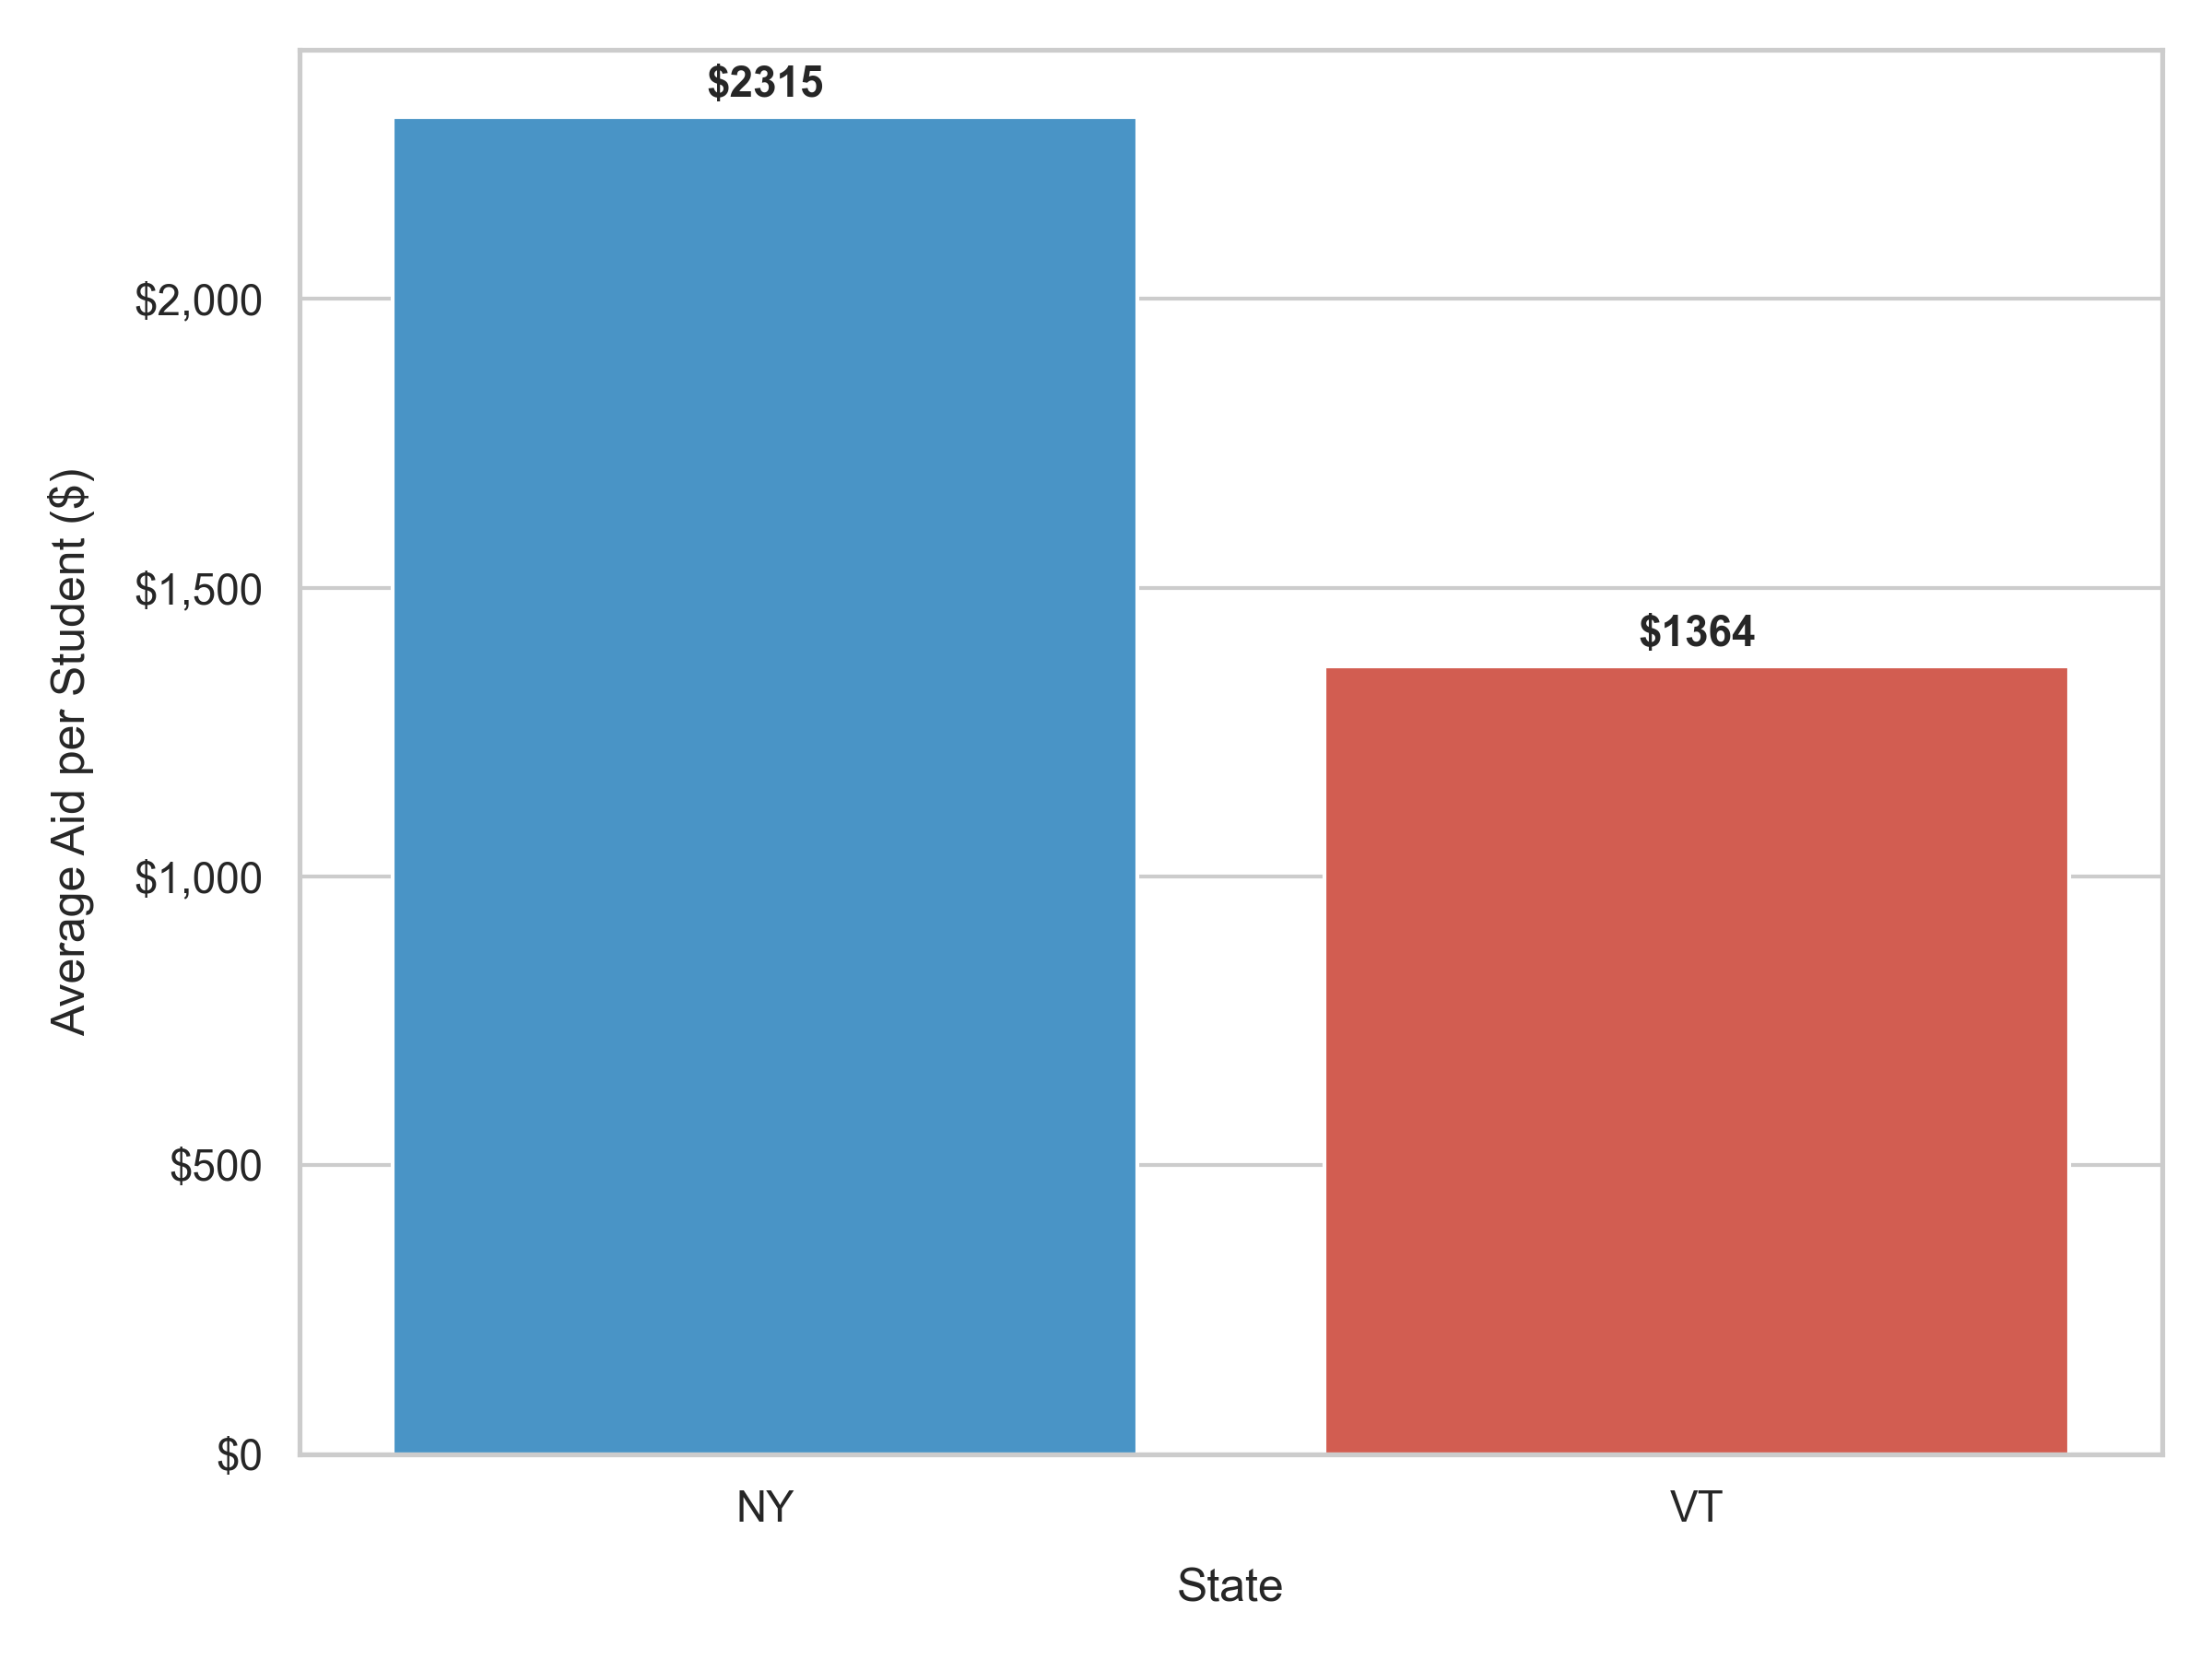
\includegraphics[width=\linewidth]{figure2_ny_vt_aid.png}
    \caption{Average Federal Grant Aid per Student: New York vs. Vermont (\AidAcademicYear)}
    \label{fig:ny-vt}
\end{figure}

\begin{figure}[htbp]
    \centering
    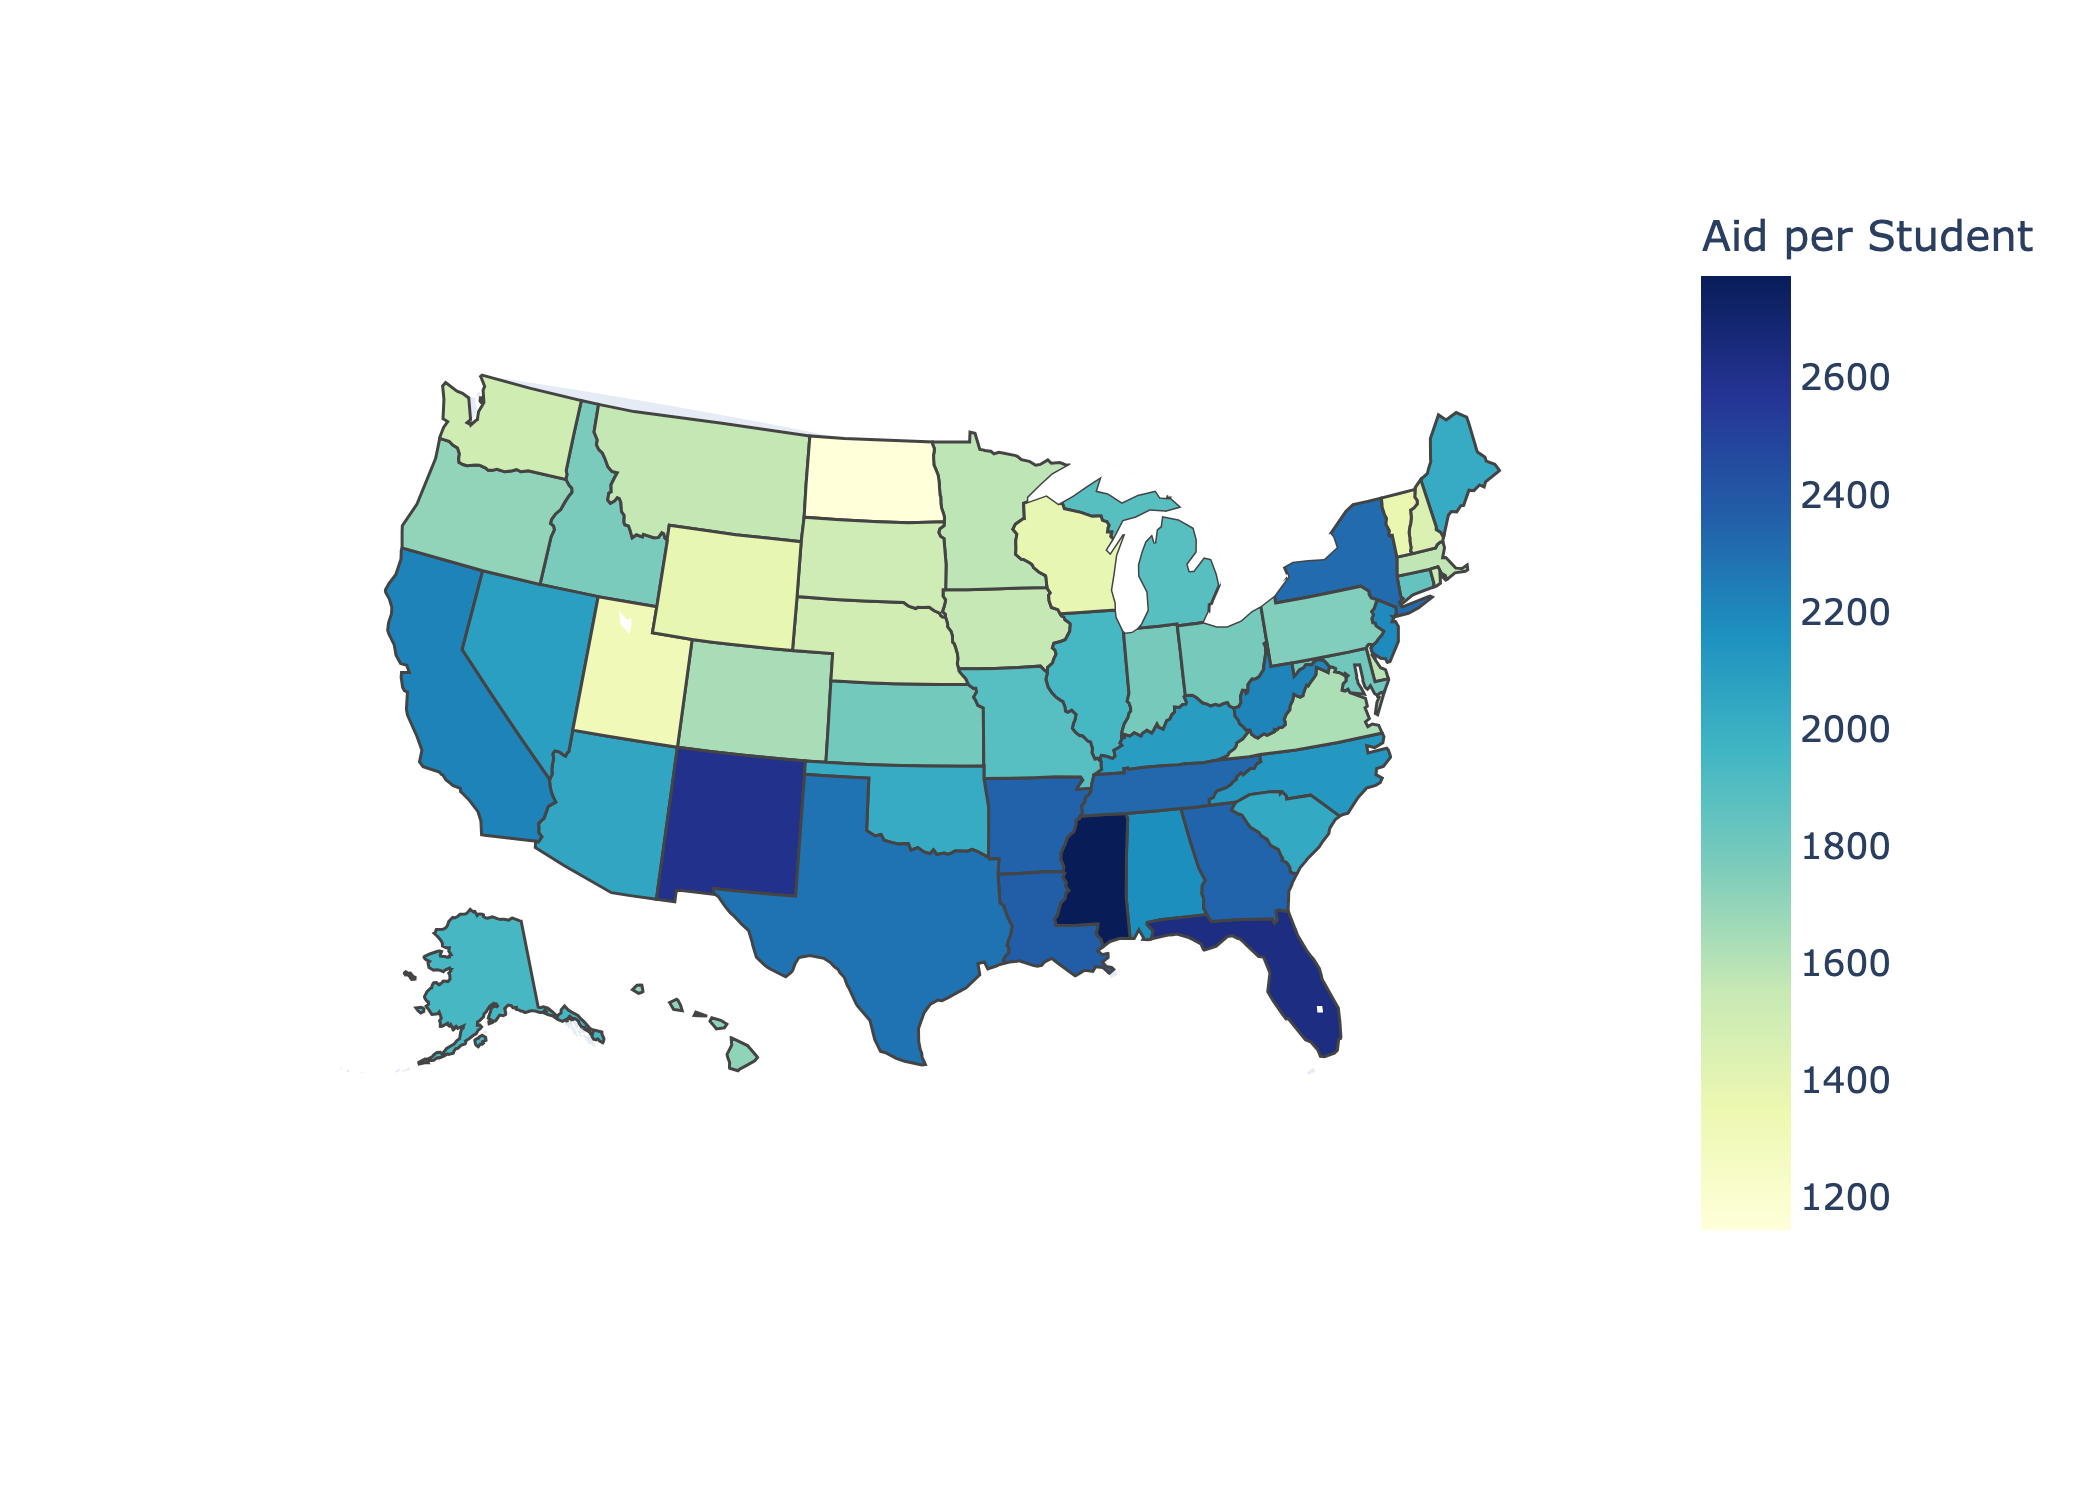
\includegraphics[width=\linewidth]{figure3_state_aid_map.png}
    \caption{Average Federal Grant Aid per Student by State (\AidAcademicYear)}
    \label{fig:state-aid}
\end{figure}

\begin{figure}[htbp]
    \centering
    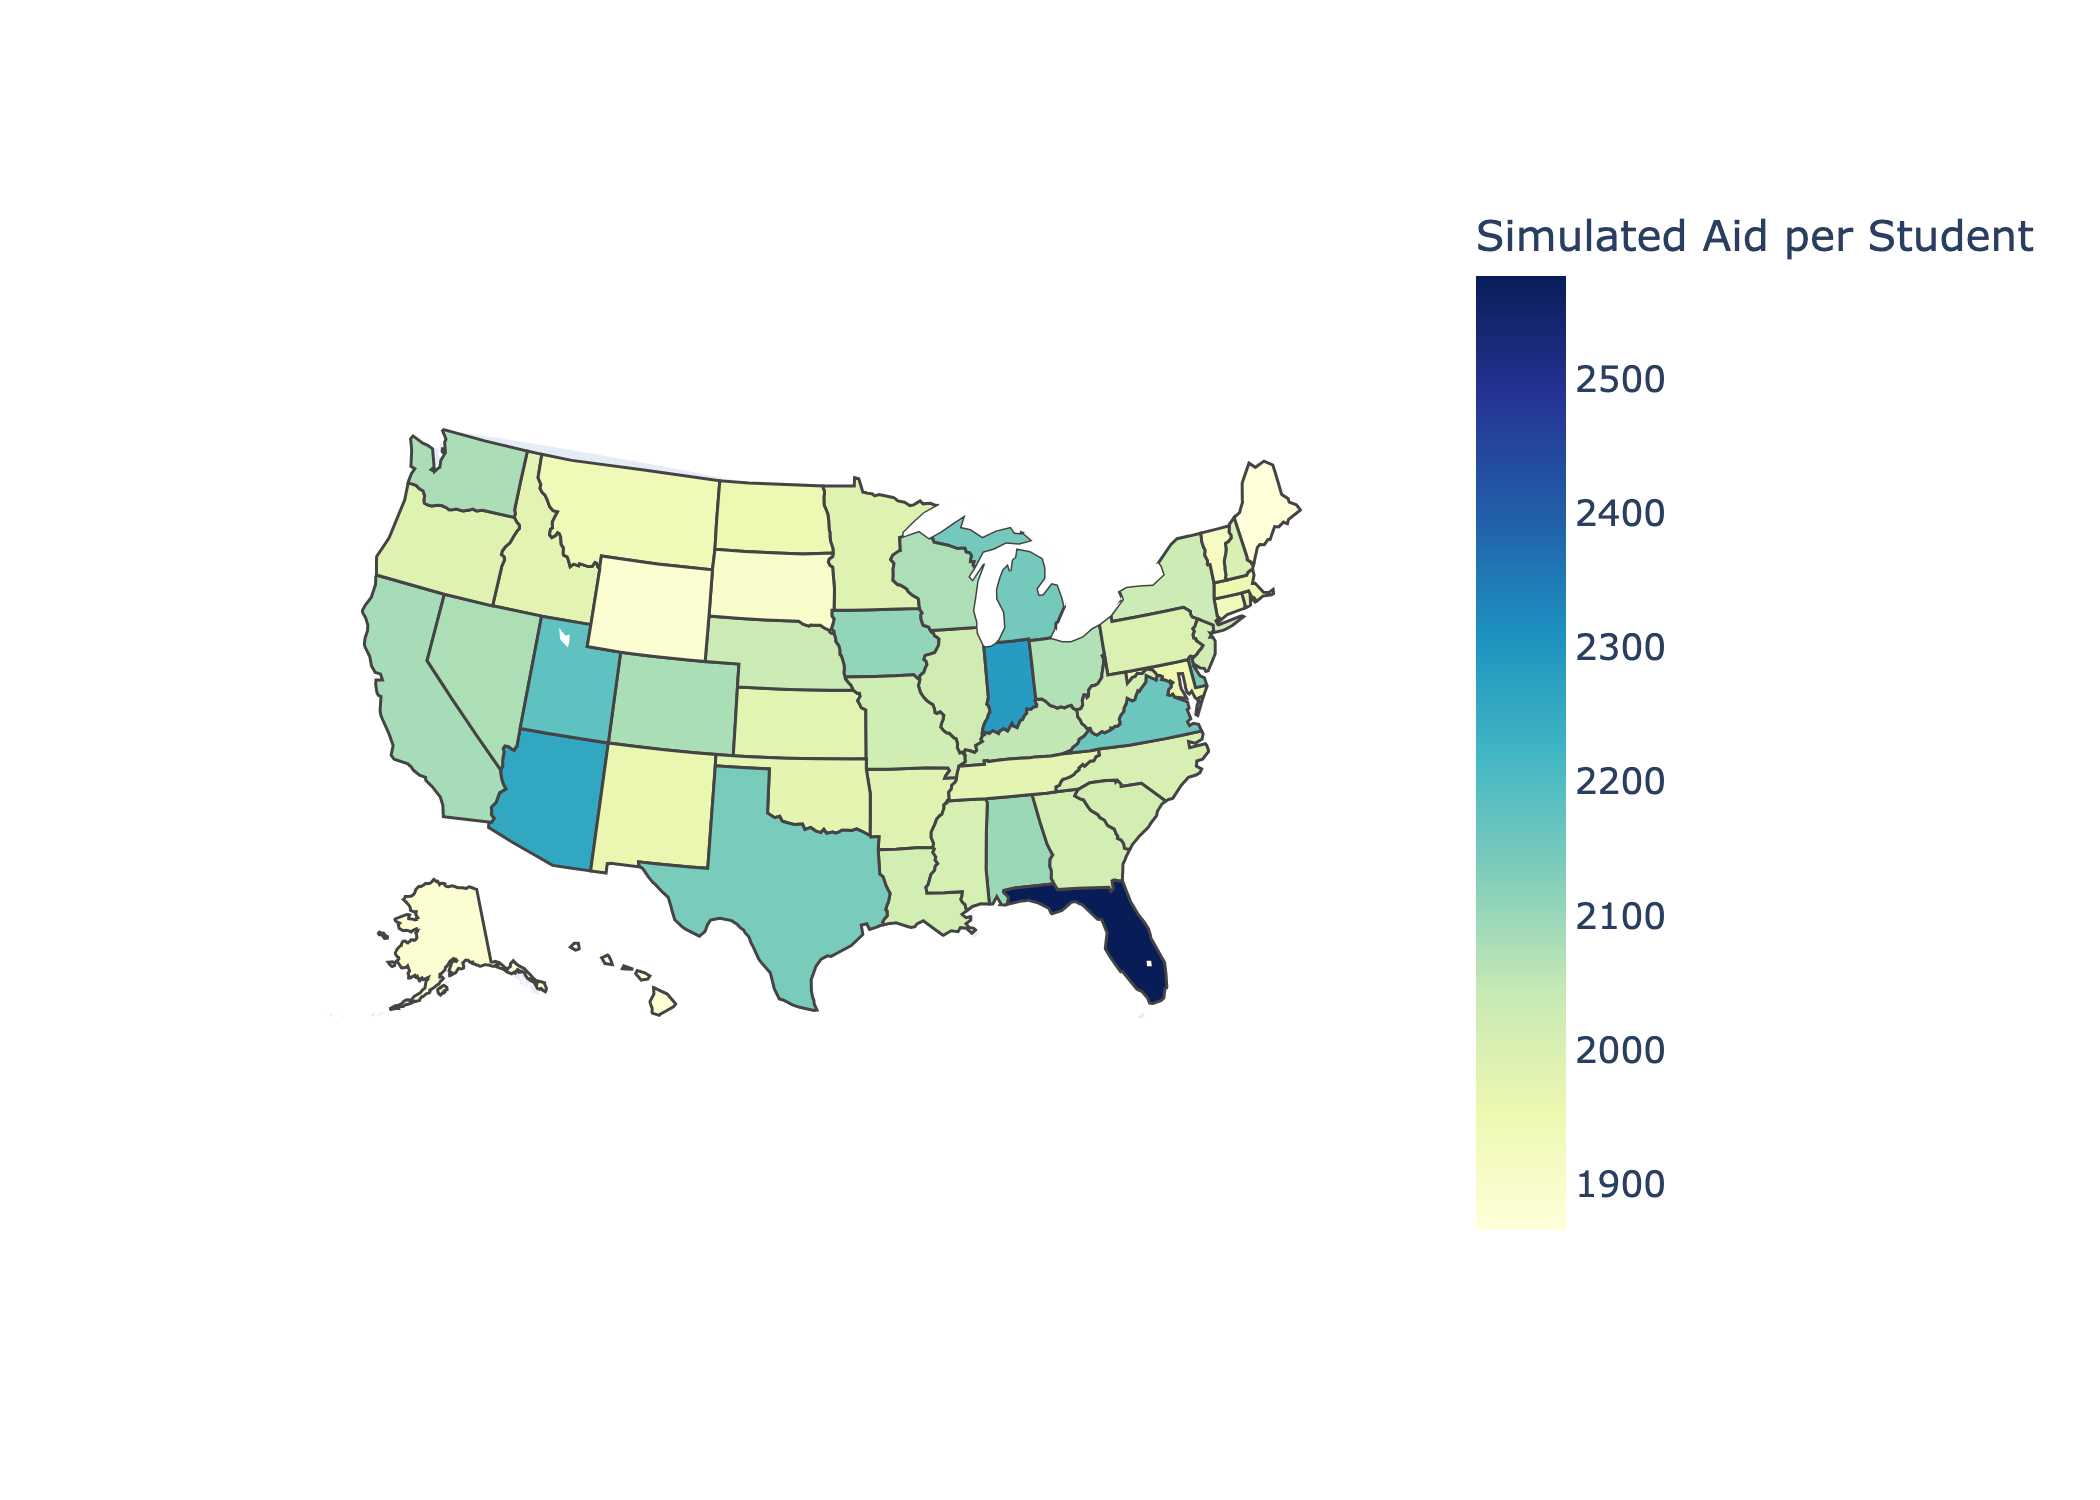
\includegraphics[width=\linewidth]{figure4_simulated_aid_map.png}
    \caption{Simulated Federal Grant Aid per Student by State}
    \label{fig:simulated-aid}
\end{figure}

\begin{figure}[htbp]
    \centering
    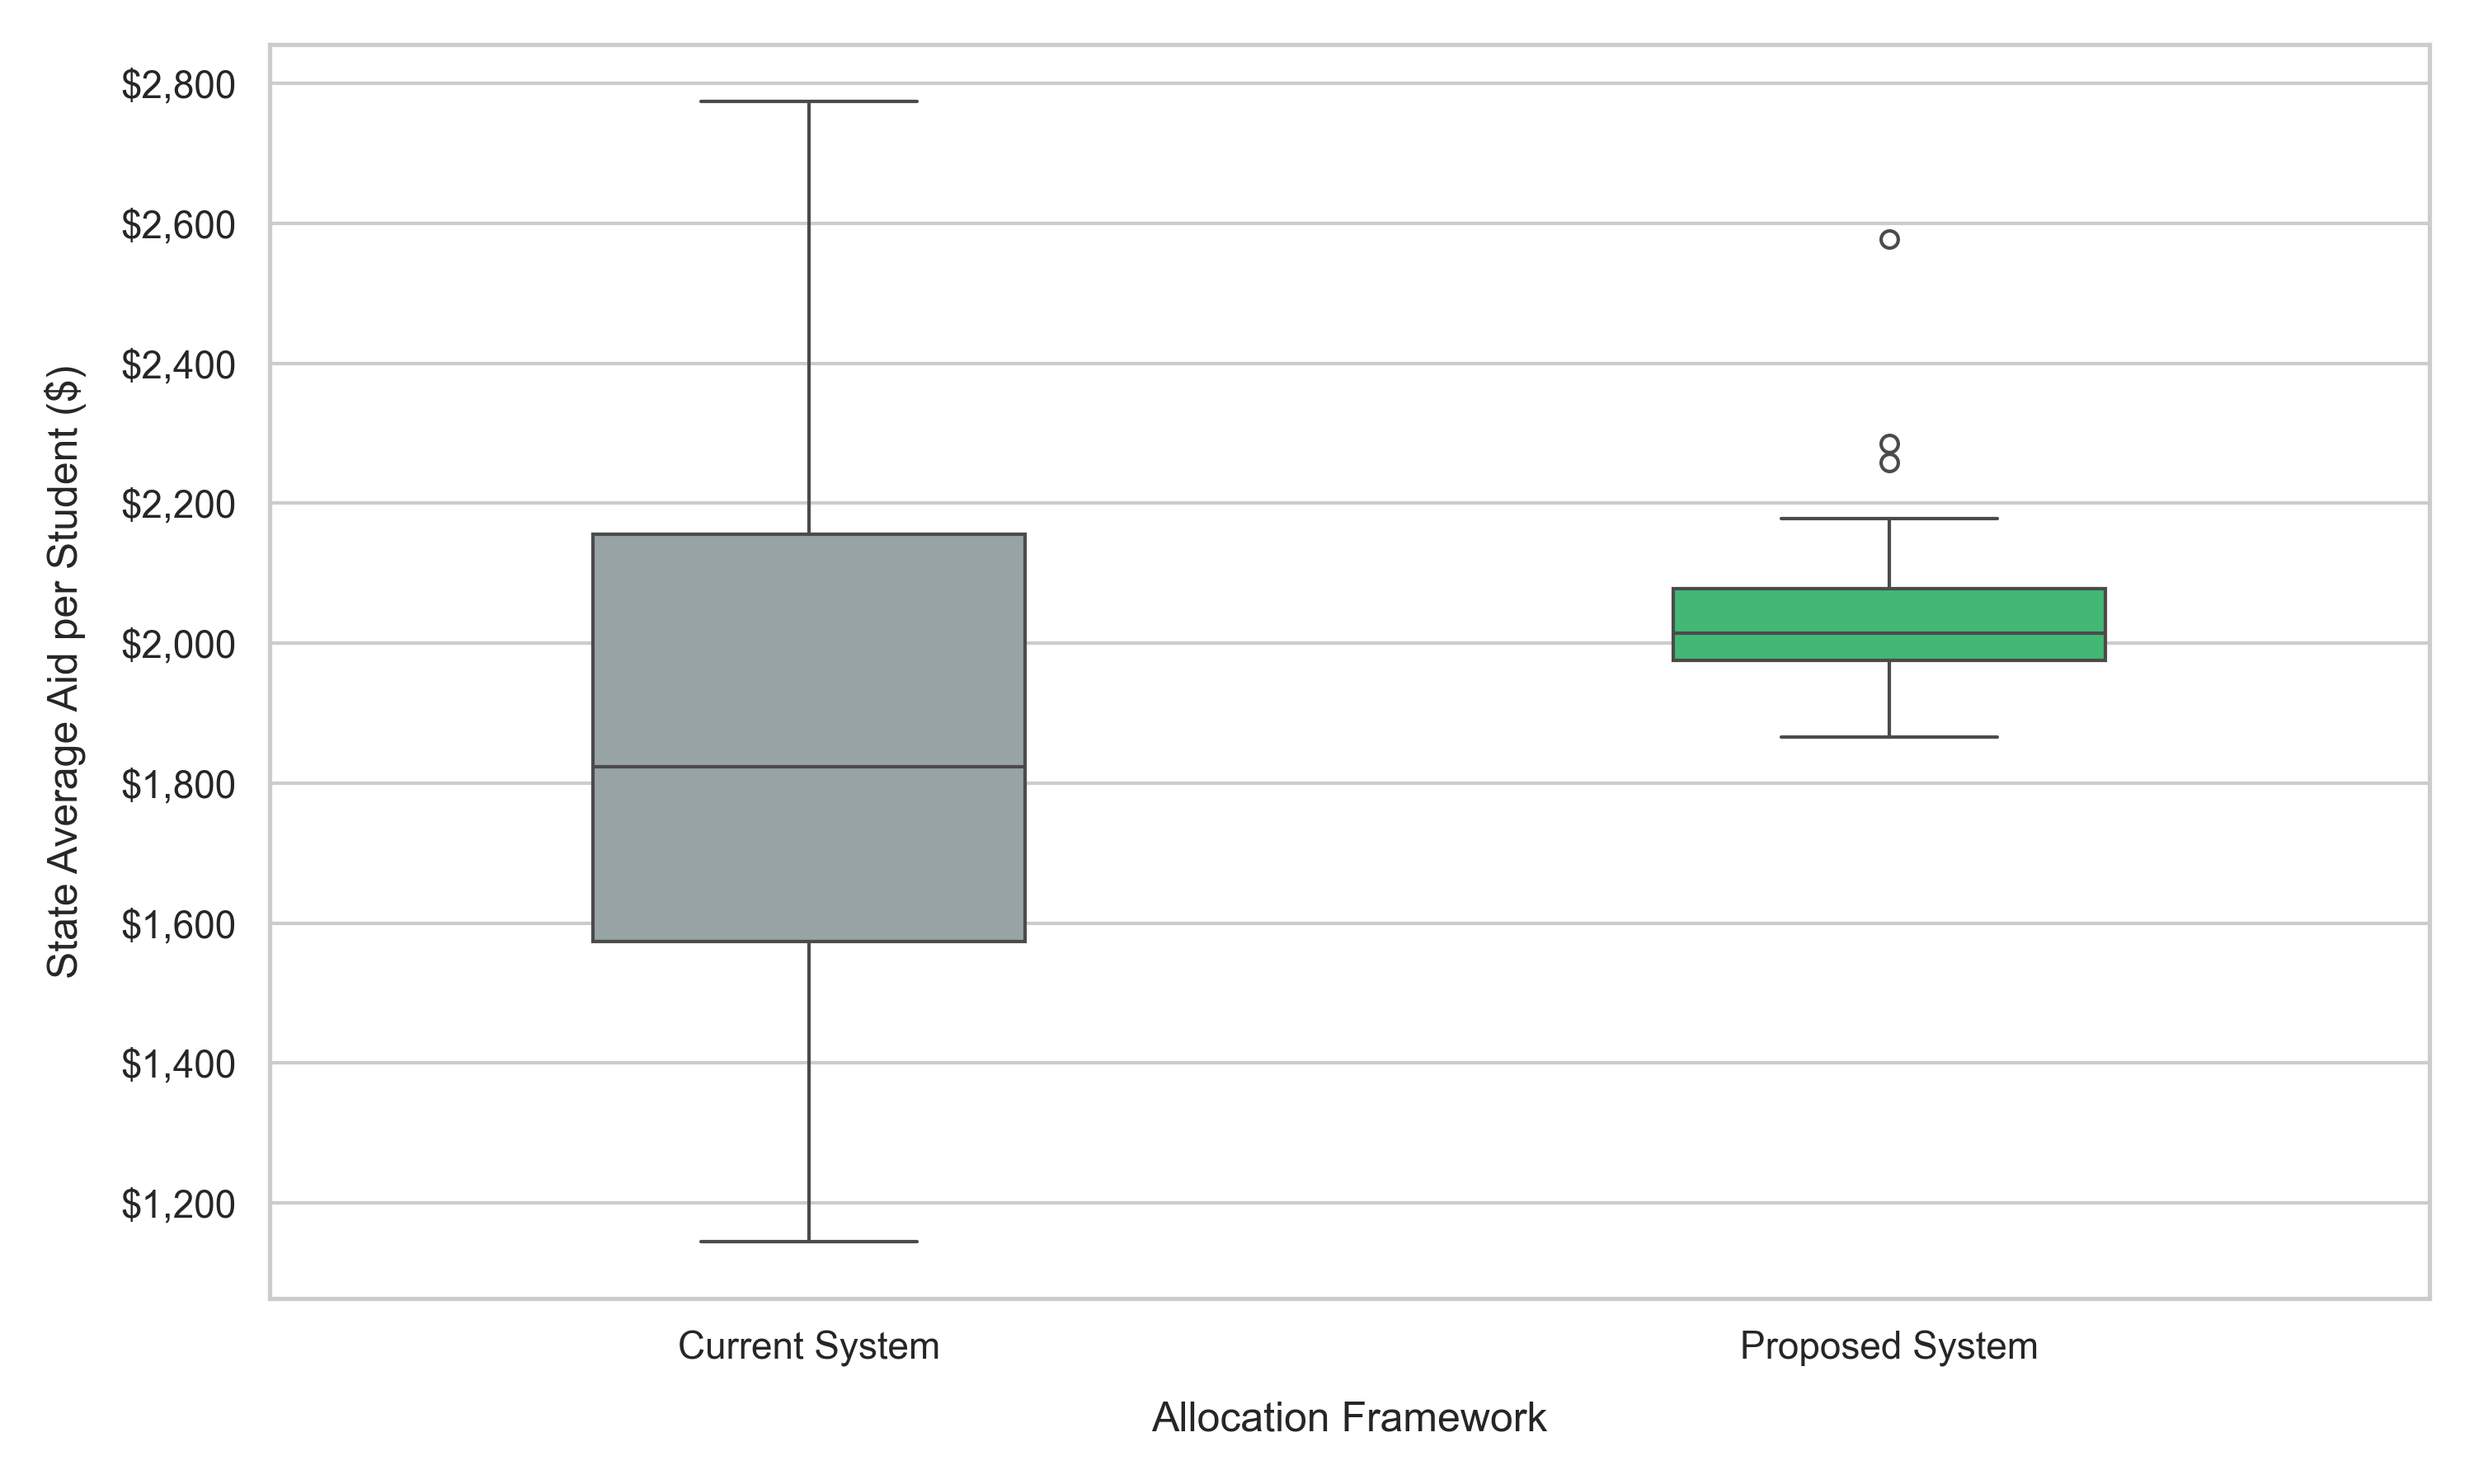
\includegraphics[width=\linewidth]{figure5_policy_simulation.png}
    \caption{Distribution of State Average Per-Student Aid: Observed and Simulated (\AidAcademicYear)}
    \label{fig:policy-spread}
\end{figure}

\begin{figure}[htbp]
    \centering
    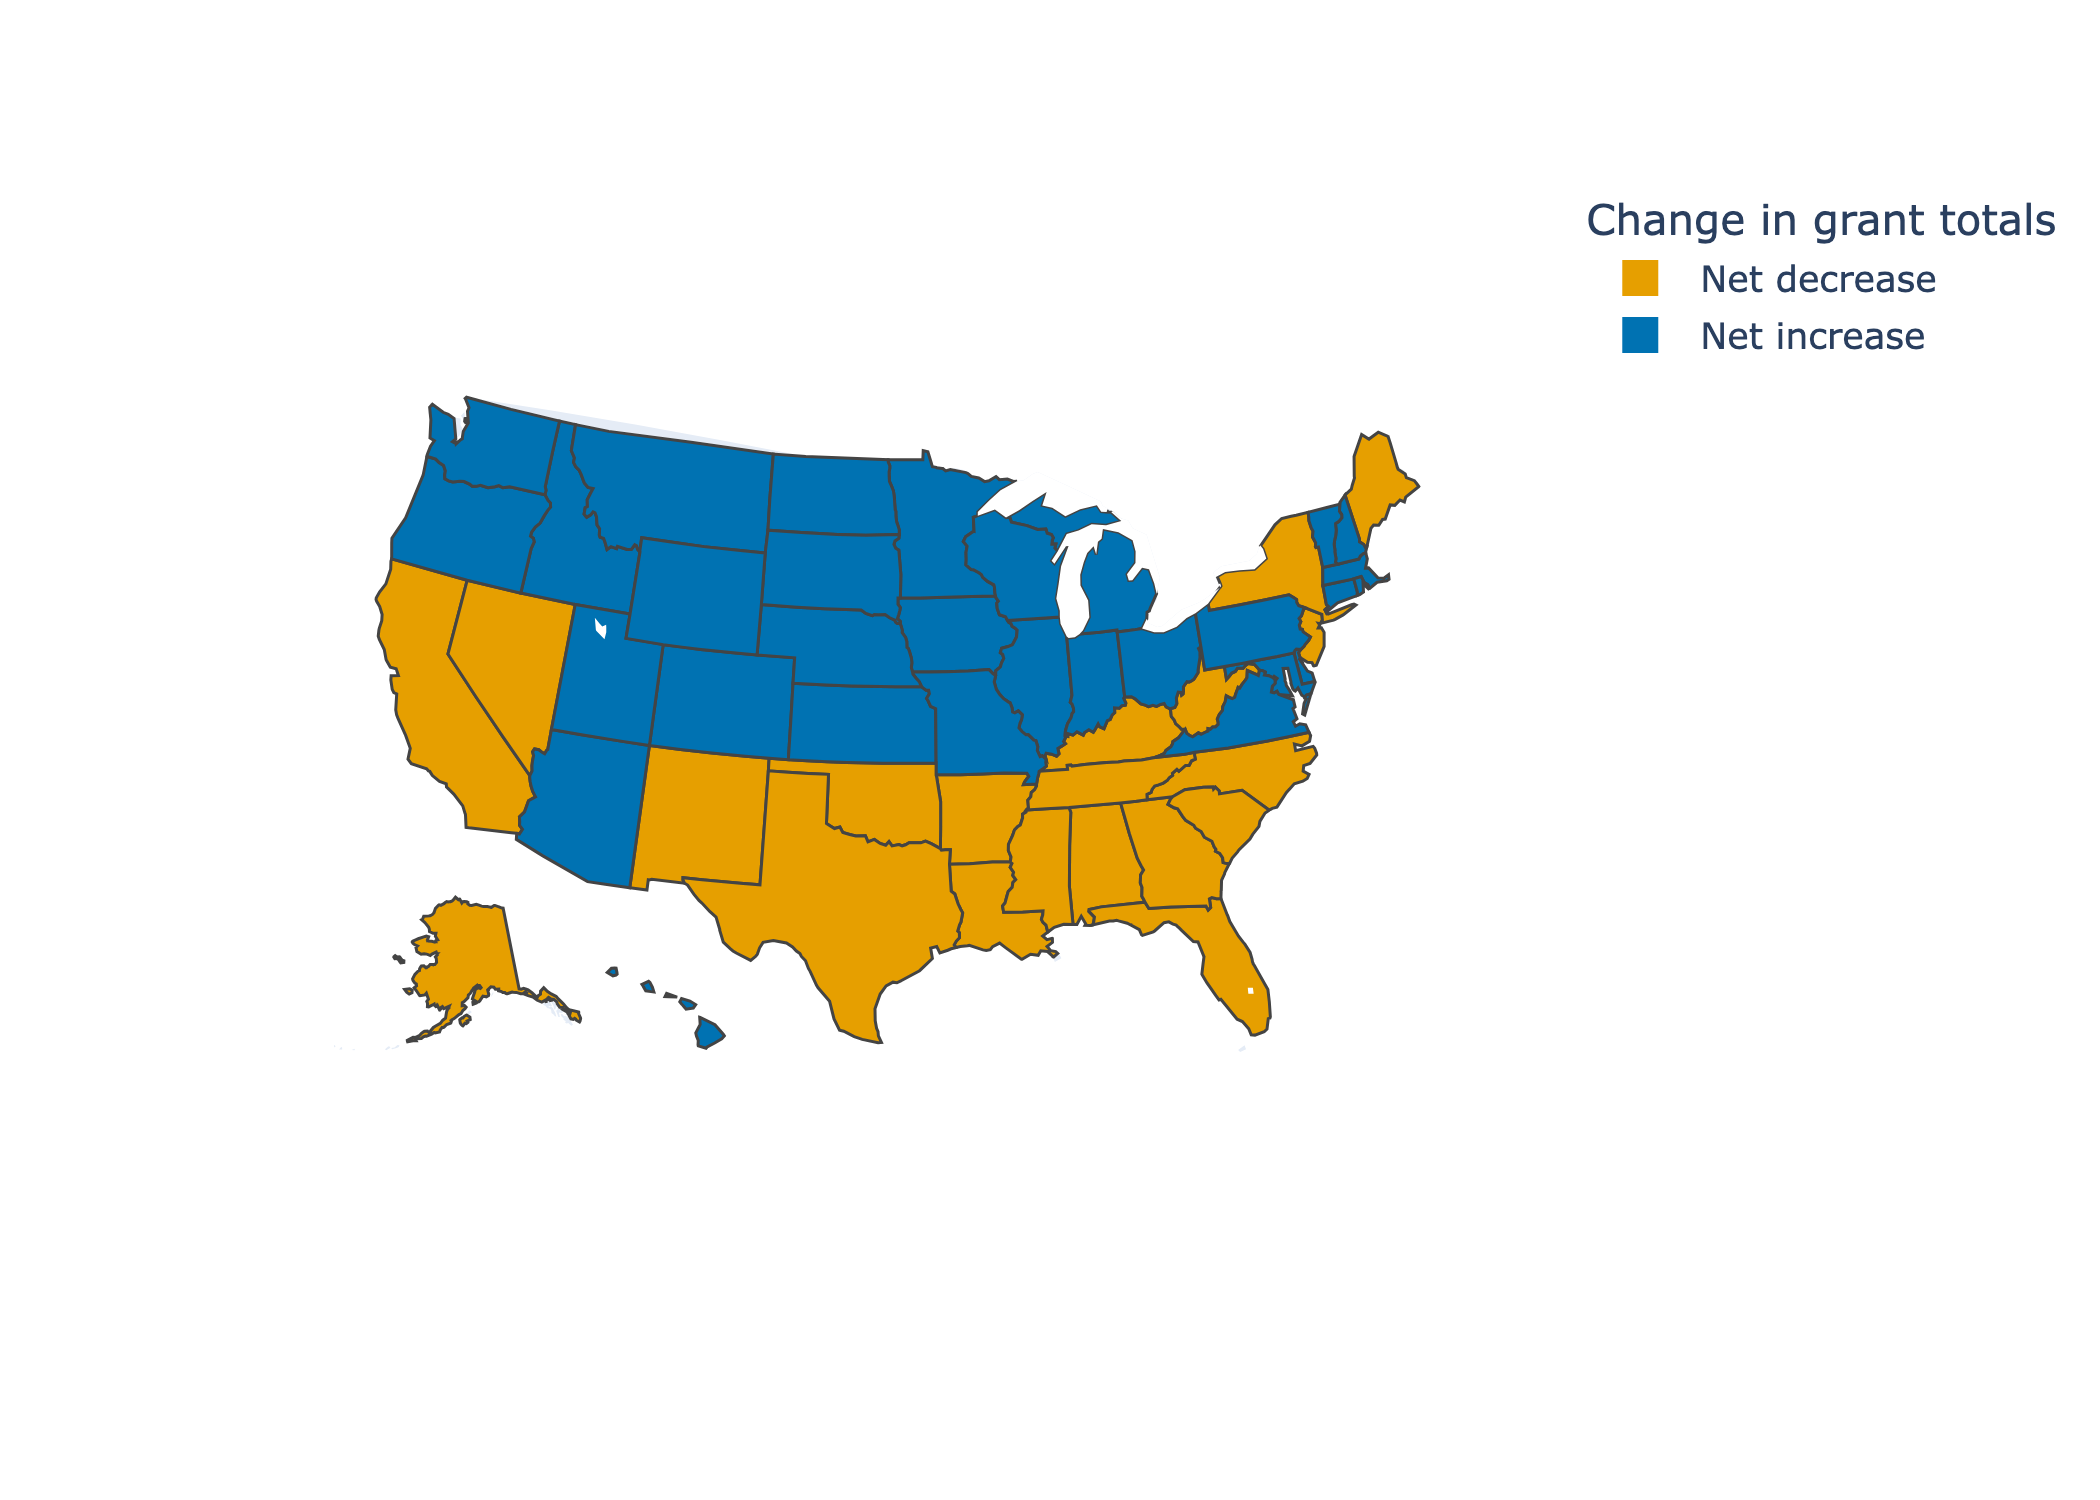
\includegraphics[width=\linewidth]{figure6_winners_losers_map.png}
    \caption{States with Increases and Decreases in Simulated Grant Totals}
    \label{fig:winners-losers}
\end{figure}
\end{document}
